\documentclass{article}
\usepackage{graphicx}
\usepackage{caption}
\usepackage{geometry}
\usepackage{placeins}
\usepackage{enumitem}
\usepackage{tcolorbox}
\usepackage{multirow}
\usepackage{float}

% Set page margins
\geometry{a4paper, margin=2cm}

% Set paragraph and spacing
\setlength{\parindent}{0em} % No indentation (annoying)
\setlength{\parskip}{0.5em} % Small space between paragraph

% Redefine the caption format to remove "Figure *:"
\captionsetup[figure]{labelformat=empty}

\begin{document}

\title{PAR - Assignment 2 - Report}
\author{\normalsize Bruno Sánchez \& Jean Dié}
\date{\small 5th November 2024}

\maketitle

\section{Introduction to the Problem}

This assignment involves designing a plan for a robot chef operating in a restaurant’s kitchen to perform meal preparation tasks. The robot’s objective is to receive orders, gather necessary ingredients, execute cooking processes, and serve finished dishes. Working within a divided kitchen layout, the robot must navigate through designated areas for storage, preparation, cooking, and dishwashing while adhering to specific operational constraints.

The planning solution is implemented in the Planning Domain Definition Language (PDDL), defining actions, predicates, and conditions necessary for the robot to achieve its goals efficiently. This report includes an analysis of the problem, an overview of the PDDL implementation, test cases, and results highlighting the robot’s ability to adapt to various scenarios, manage resources, and optimize task sequences. The following sections delve into the detailed problem analysis, solution architecture, and results of scenario-based testing to evaluate the robot’s performance and adaptability.

\section{Problem Analysis}

To implement the model in \textit{PDDL}, we first need to define the predicates and actions that will be used. The model involves a chef robot operating within a grid-based kitchen layout, where it must cook and serve different kinds of dishes. The predicates define the state of the world (in this case, the kitchen and its elements), such as valid rooms and their adjacencies, the location of tools, and the condition of ingredients. Actions describe the possible operations the robot can perform, including moving around the kitchen, picking up items (tools, ingredients and dishes), and using them to assemble the required dishes. Additionally, the model must account for the relative priority of the orders and the limited amounts of ingredients.

\vspace{1em}

\begin{figure}[H]
    \centering
    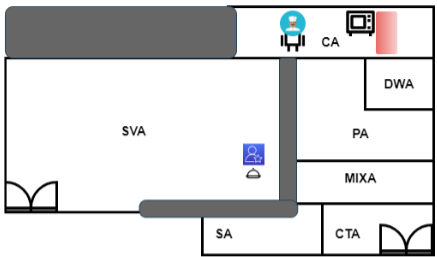
\includegraphics[width=0.55\textwidth]{assets/kitchen-layout.png}
    \caption{Kitchen layout}
    \label{fig:kitchen}
\end{figure}
\newpage
\subsection{Predicates}\label{sec:pred}

\begin{itemize}[label=--, itemsep=0.05em]
    \item \textbf{at(Movable, Room):} A \textit{Movable} entity is located in \textit{Room}.
    \item \textbf{holding(Item):} The robot is currently holding \textit{Item}.
    \item \textbf{hand-free():} The robot's hand is free.
    \item \textbf{adjacent(Room1, Room2):} \textit{Room1} and \textit{Room2} are adjacent.
    \item \textbf{ingredient-stored(Ingredient):} \textit{Ingredient} is stored in the storage area.
    \item \textbf{ingredient-available(Ingredient):} \textit{Ingredient} is available somewhere in the kitchen.
    \item \textbf{ingredient-prepared(Ingredient):} \textit{Ingredient} is prepared.
    \item \textbf{ingredient-cooked(Ingredient):} \textit{Ingredient} is cooked.
    \item \textbf{is-storage-room(Room):} \textit{Room} is designated as the storage room.
    \item \textbf{is-cooking-room(Room):} \textit{Room} is designated as the cooking room.
    \item \textbf{is-serving-room(Room):} \textit{Room} is designated as the serving room.
    \item \textbf{is-preparation-room(Room):} \textit{Room} is designated as the preparation room.
    \item \textbf{is-dishwashing-room(Room):} \textit{Room} is designated as the dishwashing room.
    \item \textbf{is-cutting-room(Room):} \textit{Room} is designated as the cutting room.
    \item \textbf{is-mixing-room(Room):} \textit{Room} is designated as the mixing room.
    \item \textbf{tool-use-room(Tool, Room):} \textit{Tool} is used in \textit{Room}.
    \item \textbf{tool-clean(Tool):} \textit{Tool} is clean.
    \item \textbf{ingredient-prep-room(Ingredient, Room):} \textit{Ingredient} must be prepared in \textit{Room}.
    \item \textbf{ingredient-used-in-dish(Ingredient, Dish):} \textit{Ingredient} is used in \textit{Dish}.
    \item \textbf{require-prepared(Dish, Ingredient):} \textit{Dish} requires \textit{Ingredient} to be prepared.
    \item \textbf{require-cooked(Dish, Ingredient):} \textit{Dish} requires \textit{Ingredient} to be cooked.
    \item \textbf{prioritize-dish(Dish1, Dish2):} \textit{Dish1} has a higher priority than \textit{Dish2}.
    \item \textbf{next-dish(Dish):} \textit{Dish} is currently being cooked.
    \item \textbf{dish-prepared(Dish):} \textit{Dish} is fully prepared.
    \item \textbf{dish-served(Dish):} \textit{Dish} has been served.
    
\end{itemize}

\subsection{Actions}\label{sec:act}

\begin{itemize}[label=--, itemsep=0.05em]
    \item \textbf{move(Robot, From, To):} \textit{Robot} moves from room \textit{From} to an adjacent room \textit{To}.
    \item \textbf{pick-up(Robot, Item, Room):} \textit{Robot} picks up \textit{Item} from \textit{Room}.
    \item \textbf{take-from-storage(Robot, Ingredient, Dish, Room):} \textit{Robot} retrieves \textit{Ingredient} from the storage room \textit{Room} for its use in \textit{Dish}.
    \item \textbf{refill-ingredient(Robot, Ingredient, Room):} \textit{Robot} refills \textit{Ingredient} in the storage \textit{Room}.
    \item \textbf{drop-tool(Robot, Tool, Room):} \textit{Robot} drops \textit{Tool} in \textit{Room}, its designated use room.
    \item \textbf{drop-ingredient(Robot, Ingredient, Room):} \textit{Robot} places \textit{Ingredient} in \textit{Room}, either the ingredient's preparation room or the general preparation room.
    \item \textbf{prepare-ingredient(Robot, Ingredient, Tool, Room):} \textit{Robot} prepares \textit{Ingredient} in \textit{Room} using \textit{Tool}.
    \item \textbf{cook-ingredient(Robot, Ingredient, Room):} \textit{Robot} cooks \textit{Ingredient} in the cooking \textit{Room}.
    \item \textbf{assemble-dish(Robot, Dish, Room):} \textit{Robot} assembles \textit{Dish} from prepared ingredients in the preparation \textit{Room}.
    \item \textbf{serve-dish(Robot, Room, Dish):} \textit{Robot} serves \textit{Dish} in the serving \textit{Room}.
    \item \textbf{clean-tool(Robot, Tool, Room):} \textit{Robot} cleans \textit{Tool} in the dishwashing \textit{Room}.
    \end{itemize}

\section{Project Structure and PDDL Implementation}

The project is mainly contained in the \texttt{code} directory, which contains the necessary files for implementing and testing the model. It includes a \texttt{domain.pddl} file, which establishes the model's conditions, including predicates and actions; and the \texttt{problem-*.pddl} files, which define the initial conditions and goal states for each test case, allowing us to evaluate the model under various scenarios.

Additionally, each problem has a corresponding \texttt{problem-*.plan} file, which contains the PDDL plan generated by the planner, and a \texttt{problem-*.txt} file, which logs the planner's output, including computational metrics. To efficiently extract and analyze these metrics, we developed a Python script, \texttt{run\_plan.py}, which executes the planner for a chosen problem and logs its output to provide insights into the computational performance of the model.

To facilitate the development and testing of our PDDL files, we set up our project using \textbf{Visual Studio Code} with the PDDL extension. We utilized the \textbf{BFWS planner} to execute and evaluate our PDDL models, allowing us to test various scenarios and configurations efficiently.

In this section, we will only explain the \texttt{domain.pddl} implementation of the model. In the next section, \textit{Test Cases and Results}, we will show the multiple problem configurations that we have tested and the results attained with each of them.

\subsection{Requirements}
The PDDL requirements needed in the domain are:
\begin{enumerate}
    \item \texttt{:strips}, which indicates that the domain adheres to the basic action representation of the STRIPS framework.
    \item \texttt{:typing}, which allows the use of types for predicates and objects in the domain.
    \item \texttt{:negative-preconditions}, which enables the use of the \texttt{not} operator in the preconditions of actions.
    \item \texttt{:disjunctive-preconditions}, which allows for the use of the \texttt{or} operator in the preconditions of actions.
    \item \texttt{:conditional-effects}, which permits the specification of effects that depend on the state of the world, with the \texttt{when} operator.
    \item \texttt{:universal-preconditions}, which allows for preconditions that must hold for all objects of a specific type, with the \texttt{forall} operator.
    \end{enumerate}
\begin{figure}[ht]
    \centering
    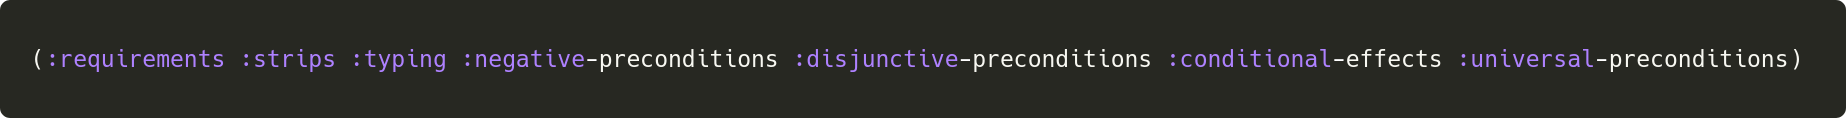
\includegraphics[width=0.90\textwidth]{assets/requirements.png}
    \caption{Code: Requirements}
    \label{fig:req}
\end{figure}

\subsection{Types}
The types are used to categorize objects within a domain, providing a way to define relationships and constraints between different entities.
\begin{enumerate}
    \item \texttt{room - object}, which defines a type for locations or rooms.
    \item \texttt{movable - object}, which defines a type for movable entities.
    \item \texttt{robot - movable}, which specifies that the robot is a type of movable object.
    \item \texttt{item - movable}, which defines a general type `item' for anything the robot might hold.
    \item \texttt{ingredient, tool, dish - item}, which specifies that `ingredient', `tool', and `dish' are subtypes of `item'.    
\end{enumerate}
\begin{figure}[H]
    \centering
    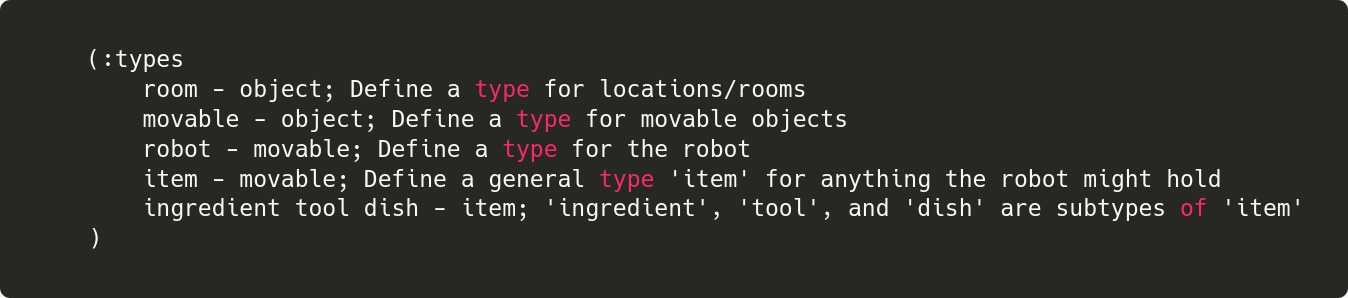
\includegraphics[width=0.90\textwidth]{assets/types.jpeg}
    \caption{Code: Types}
    \label{fig:types}
\end{figure}

\subsection{Predicates}
The predicates are essentially variables that can take either a \textit{true} or \textit{false} value for each collection of \textit{parameters} that they are given. In our domain, the predicates are those discussed in Section~\ref{sec:pred}.
\begin{figure}[H]
    \centering
    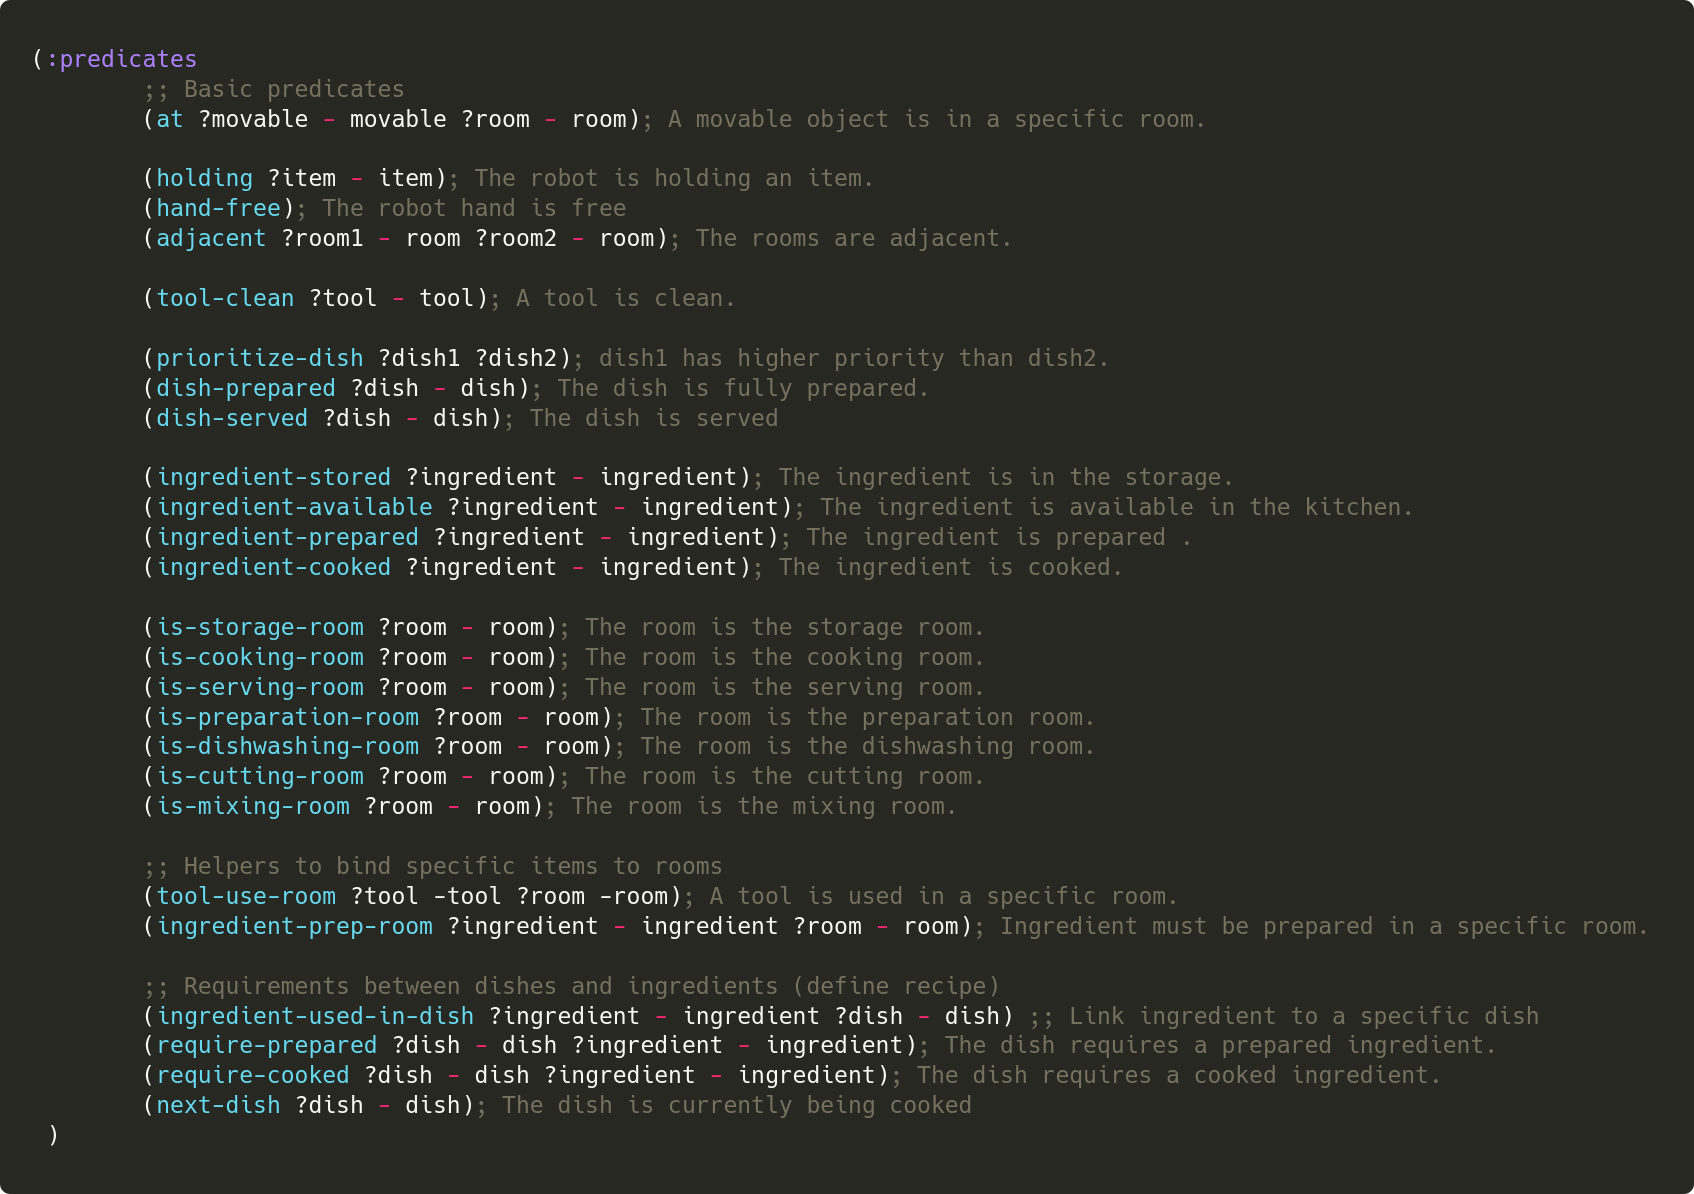
\includegraphics[width=0.90\textwidth]{assets/predicates.png}
    \caption{Code: Predicates}
    \label{fig:pred}
\end{figure}

\subsection{Actions}
The actions are the possible steps that can be taken throughout a plan. Each of them recieves a number of \textit{parameters}, which are the objects that intervene in the action. Then, for the action to be allowed to happen, all of its \textit{preconditions} have to be met and, in that case, the \textit{effects} of the action can be applied. In our domain, the actions are those discussed in Section~\ref{sec:act}.
\subsubsection{Move}
The \texttt{move} action allows the robot to move between adjacent rooms of the kitchen.
\begin{itemize}
    \item \underline{Parameters:}
    \begin{itemize}
        \item \texttt{Robot}: The robot that is performing the move action.
        \item \texttt{From}: The room from which the robot is moving.
        \item \texttt{To}: The room to which the robot is moving.
    \end{itemize}
    \item \underline{Preconditions:}
    \begin{itemize}
        \item \textit{At(Robot, From)}: The robot must be located in the room \texttt{From}.
        \item \textit{Adjacent(From, To)}: The rooms \texttt{From} and \texttt{To} must be adjacent to each other.
    \end{itemize}
    \item \underline{Effects:}
    \begin{itemize}
        \item \textit{At(Robot, To)}: The robot is now located in the room \texttt{To}.
        \item \textit{¬At(Robot, From)}: The robot is no longer in the room \texttt{From}.
    \end{itemize}
\end{itemize}
\begin{figure}[ht]
    \centering
    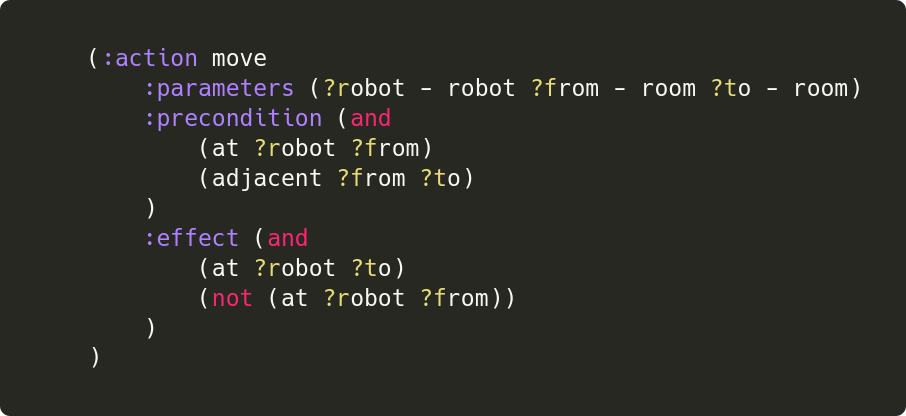
\includegraphics[width=0.80\textwidth]{assets/move.png}
    \caption{Code: Move Action}
    \label{fig:act:move}
\end{figure}

\subsubsection{Pick-up}
The \texttt{pick-up} action allows the robot to take items (tools, ingredients or dishes) from the kitchen.

\begin{itemize}
    \item \underline{Parameters:}
    \begin{itemize}
        \item \texttt{Robot}: The robot that is performing the pick-up action.
        \item \texttt{Item}: The item that the robot intends to pick up.
        \item \texttt{Room}: The room where the robot and the item are located.
    \end{itemize}
    \item \underline{Preconditions:}
    \begin{itemize}
        \item \textit{At(Robot, Room)}: The robot must be located in the room \texttt{Room}.
        \item \textit{At(Item, Room)}: The item must also be located in the same room \texttt{Room}.
        \item \textit{Hand-free}: The robot must not be holding any other item.
    \end{itemize}
    \item \underline{Effects:}
    \begin{itemize}
        \item \textit{Holding(Item)}: The robot is now holding the item \texttt{Item}.
        \item \textit{¬Hand-free}: The robot's hand is no longer free (it is now holding an item).
        \item \textit{¬At(Item, Room)}: The item is no longer located in the room \texttt{Room}.
    \end{itemize}
\end{itemize}
\begin{figure}[ht]
    \centering
    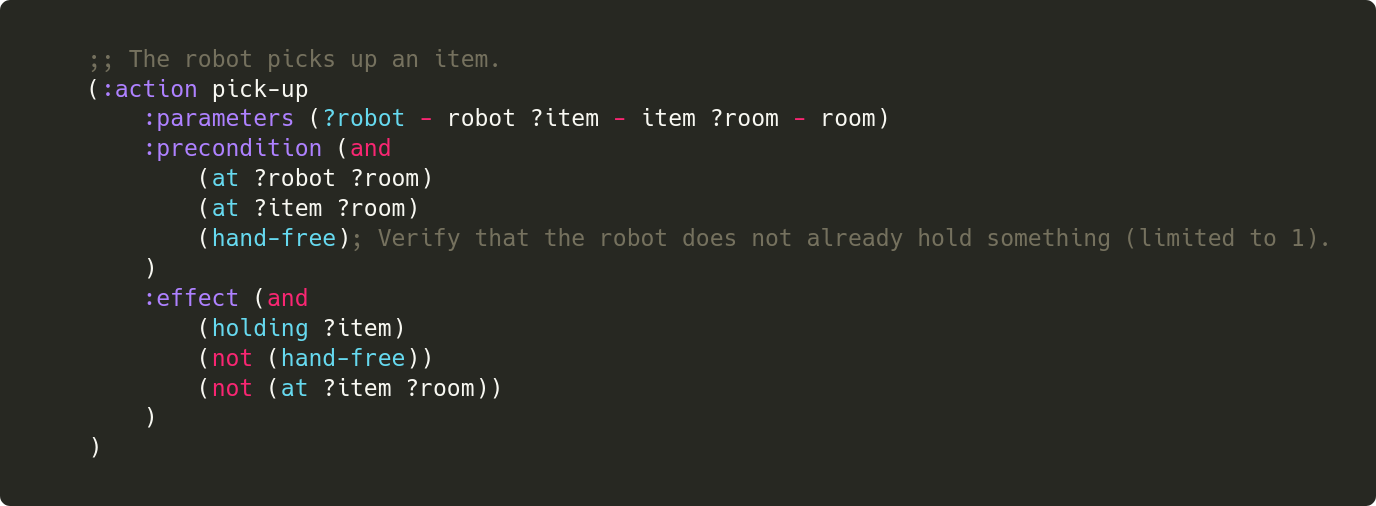
\includegraphics[width=0.90\textwidth]{assets/pick-up.png}
    \caption{Code: Pick-Up Action}
    \label{fig:act:pick-up}
\end{figure}

\subsubsection{Take-from-storage}
The \texttt{take-from-storage} action allows the robot to take an ingredient from the storage and make it available in the kitchen.
\begin{itemize}
    \item \underline{Parameters:}
    \begin{itemize}
        \item \texttt{Robot}: The robot that is performing the take-from-storage action.
        \item \texttt{Ingredient}: The ingredient that the robot intends to take from storage.
        \item \texttt{Dish}: The dish that requires the ingredient.
        \item \texttt{Room}: The room where the robot and the storage are located.
    \end{itemize}
    \item \underline{Preconditions:}
    \begin{itemize}
        \item \textit{At(Robot, Room)}: The robot must be located in the room \texttt{Room}.
        \item \textit{Is-storage-room(Room)}: The room must be designated as a storage room.
        \item \textit{Ingredient-stored(Ingredient)}: The ingredient must currently be stored in the storage room.
        \item \textit{Hand-free}: The robot must not be holding any other item.
        \item \textit{Next-dish(Dish)}: The dish must be the next one to be prepared.
        \item \textit{Ingredient-used-in-dish(Ingredient, Dish)}: The ingredient must be required for the specified dish.
    \end{itemize}
    \item \underline{Effects:}
    \begin{itemize}
        \item \textit{Holding(Ingredient)}: The robot is now holding the ingredient \texttt{Ingredient}.
        \item \textit{Ingredient-available(Ingredient)}: The ingredient is now available for use.
        \item \textit{¬Hand-free}: The robot's hand is no longer free (it is now holding an ingredient).
        \item \textit{¬Ingredient-stored(Ingredient)}: The ingredient is no longer in storage.
    \end{itemize}
\end{itemize}
\begin{figure}[H]
    \centering
    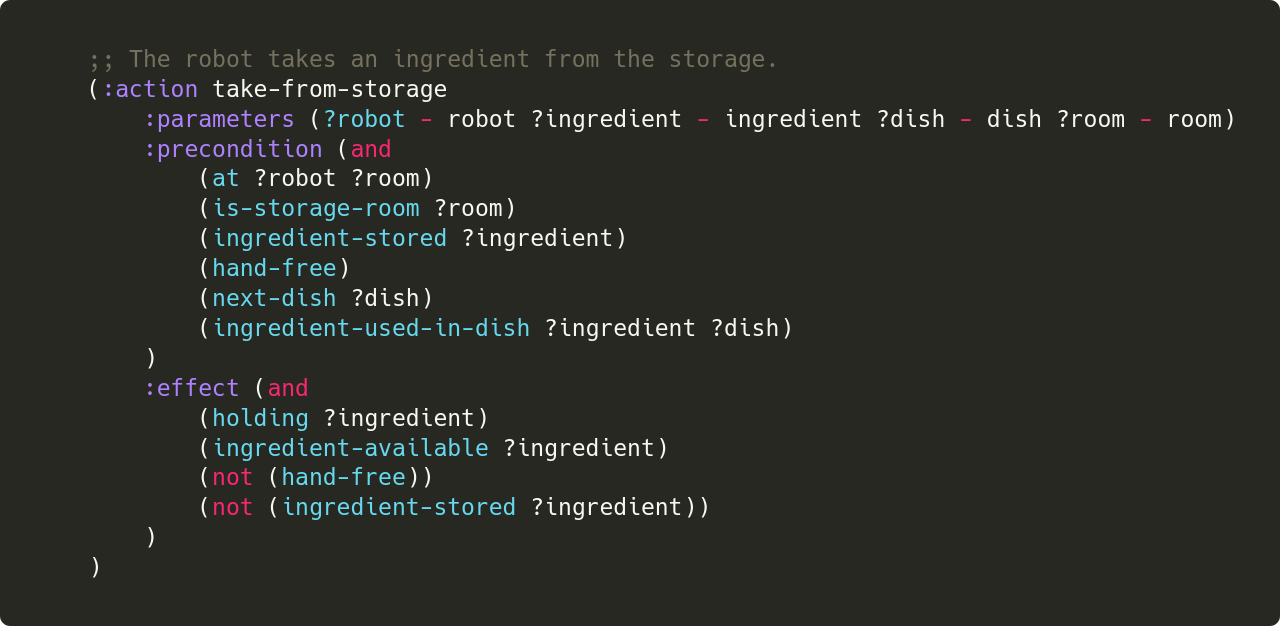
\includegraphics[width=0.90\textwidth]{assets/take-from-storage.png}
    \caption{Code: Take-from-storage Action}
    \label{fig:act:take}
\end{figure}

\subsubsection{Refill-ingredient}
The \texttt{refill-ingredient} action restocks the storage with a specific ingredient that is no longer available.
\begin{itemize}
    \item \underline{Parameters:}
    \begin{itemize}
        \item \texttt{Robot}: The robot that is performing the refill action.
        \item \texttt{Ingredient}: The ingredient that the robot is refilling in storage.
        \item \texttt{Room}: The room where the robot and storage are located.
    \end{itemize}
    \item \underline{Preconditions:}
    \begin{itemize}
        \item \textit{At(Robot, Room)}: The robot must be located in the room \texttt{Room}.
        \item \textit{Is-storage-room(Room)}: The room must be designated as a storage room.
        \item \textit{¬Ingredient-stored(Ingredient)}: The ingredient must not currently be in storage.
        \item \textit{¬Ingredient-available(Ingredient)}: The ingredient must not be available in the kitchen.
    \end{itemize}
    \item \underline{Effects:}
    \begin{itemize}
        \item \textit{Ingredient-stored(Ingredient)}: The ingredient is now stored in the storage room.
    \end{itemize}
\end{itemize}
\begin{figure}[ht]
    \centering
    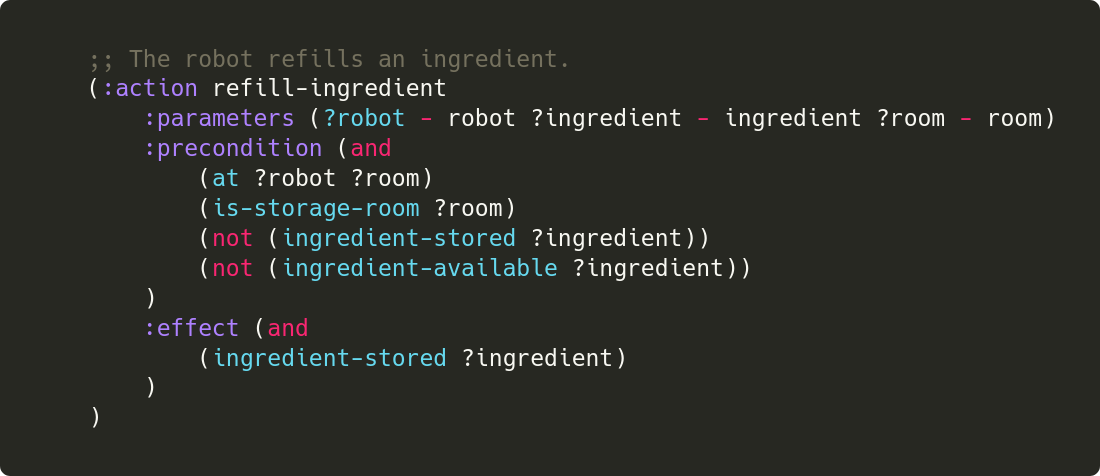
\includegraphics[width=0.80\textwidth]{assets/refill-ingredient.png}
    \caption{Code: Refill-ingredient Action}
    \label{fig:act:refill}
\end{figure}

\subsubsection{Drop-tool}
The \texttt{drop-tool} action makes the robot drop a tool. A tool can only be droped at its use room.
\begin{itemize}
    \item \underline{Parameters:}
    \begin{itemize}
        \item \texttt{Robot}: The robot performing the drop action.
        \item \texttt{Tool}: The tool that the robot intends to drop.
        \item \texttt{Room}: The room where the tool should be dropped.
    \end{itemize}
    \item \underline{Preconditions:}
    \begin{itemize}
        \item \textit{At(Robot, Room)}: The robot must be located in the room \texttt{Room}.
        \item \textit{Holding(Tool)}: The robot must be holding the tool \texttt{Tool}.
        \item \textit{Tool-use-room(Tool, Room)}: The tool must be used in the specified room \texttt{Room}.
    \end{itemize}
    \item \underline{Effects:}
    \begin{itemize}
        \item \textit{¬Holding(Tool)}: The robot is no longer holding the tool.
        \item \textit{Hand-free}: The robot’s hand is now free.
        \item \textit{At(Tool, Room)}: The tool is now located in the specified room \texttt{Room}.
    \end{itemize}
    \end{itemize}
\begin{figure}[ht]
    \centering
    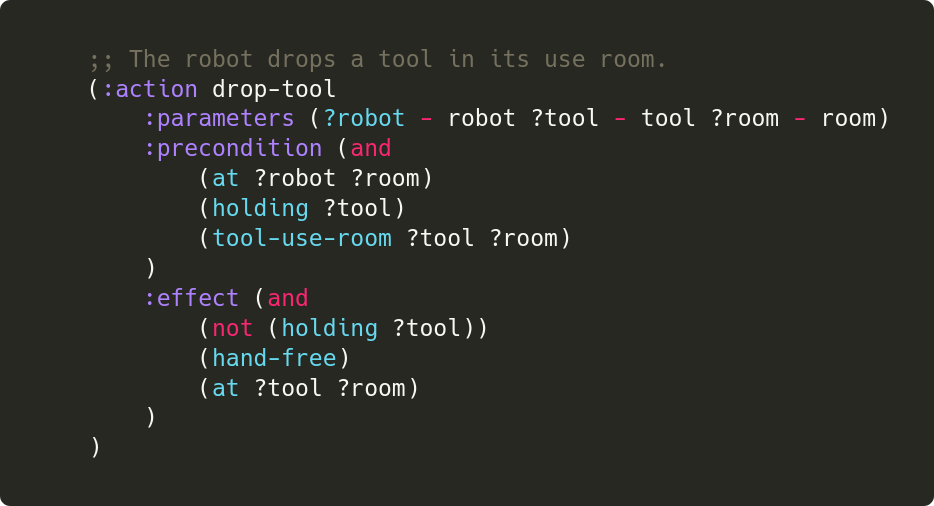
\includegraphics[width=0.80\textwidth]{assets/drop-tool.png}
    \caption{Code: Drop-tool Action}
    \label{fig:act:drop-tool}
\end{figure}

\subsubsection{Clean-tool}
The \texttt{clean-tool} action allows the robot to clean a used tool in the dishwashing room.
\begin{itemize}
    \item \underline{Parameters:}
    \begin{itemize}
        \item \texttt{Robot}: The robot responsible for cleaning the tool.
        \item \texttt{Tool}: The tool to be cleaned.
        \item \texttt{Room}: The dishwashing area where the tool is cleaned.
    \end{itemize}
    \item \underline{Preconditions:}
    \begin{itemize}
        \item \textit{At(Robot, Room)}: The robot must be located in \texttt{Room}.
        \item \textit{Is-dishwashing-room(Room)}: The room \texttt{Room} must be designated as a dishwashing area.
        \item \textit{Holding(Tool)}: The robot must be holding the tool.
        \item \textit{¬Tool-clean(Tool)}: The tool must not already be clean.
    \end{itemize}
    \item \underline{Effects:}
    \begin{itemize}
        \item \textit{Tool-clean(Tool)}: The tool is now marked as clean.
    \end{itemize}
\end{itemize}
    \begin{figure}[ht]
    \centering
    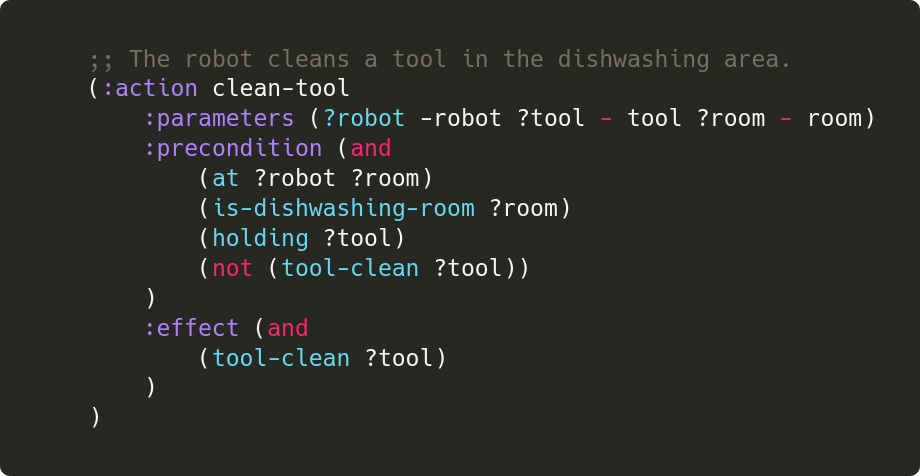
\includegraphics[width=0.75\textwidth]{assets/clean-tool.png}
    \caption{Code: Clean-tool Action}
    \label{fig:act:clean-tool}
\end{figure}

\subsubsection{Drop-ingredient}
The \texttt{drop-ingredient} action makes the robot drop an ingredient. An ingredient can only be droped at its designated preparation room or at the general preparation room.
\begin{itemize}
    \item \underline{Parameters:}
    \begin{itemize}
        \item \texttt{Robot}: The robot performing the drop action.
        \item \texttt{Ingredient}: The ingredient that the robot intends to drop.
        \item \texttt{Room}: The room where the ingredient will be dropped.
    \end{itemize}
    \item \underline{Preconditions:}
    \begin{itemize}
        \item \textit{At(Robot, Room)}: The robot must be located in the room \texttt{Room}.
        \item \textit{Holding(Ingredient)}: The robot must be holding the ingredient \texttt{Ingredient}.
        \item \textit{Ingredient-prep-room(Ingredient, Room) \textbf{or} Is-preparation-room(Room)}: The room must either be the specific preparation room for the ingredient or a designated preparation room.
    \end{itemize}
    \item \underline{Effects:}
    \begin{itemize}
        \item \textit{¬Holding(Ingredient)}: The robot is no longer holding the ingredient.
        \item \textit{Hand-free}: The robot’s hand is now free.
        \item \textit{At(Ingredient, Room)}: The ingredient is now located in the specified room \texttt{Room}.
    \end{itemize}
\end{itemize}
    \begin{figure}[ht]
    \centering
    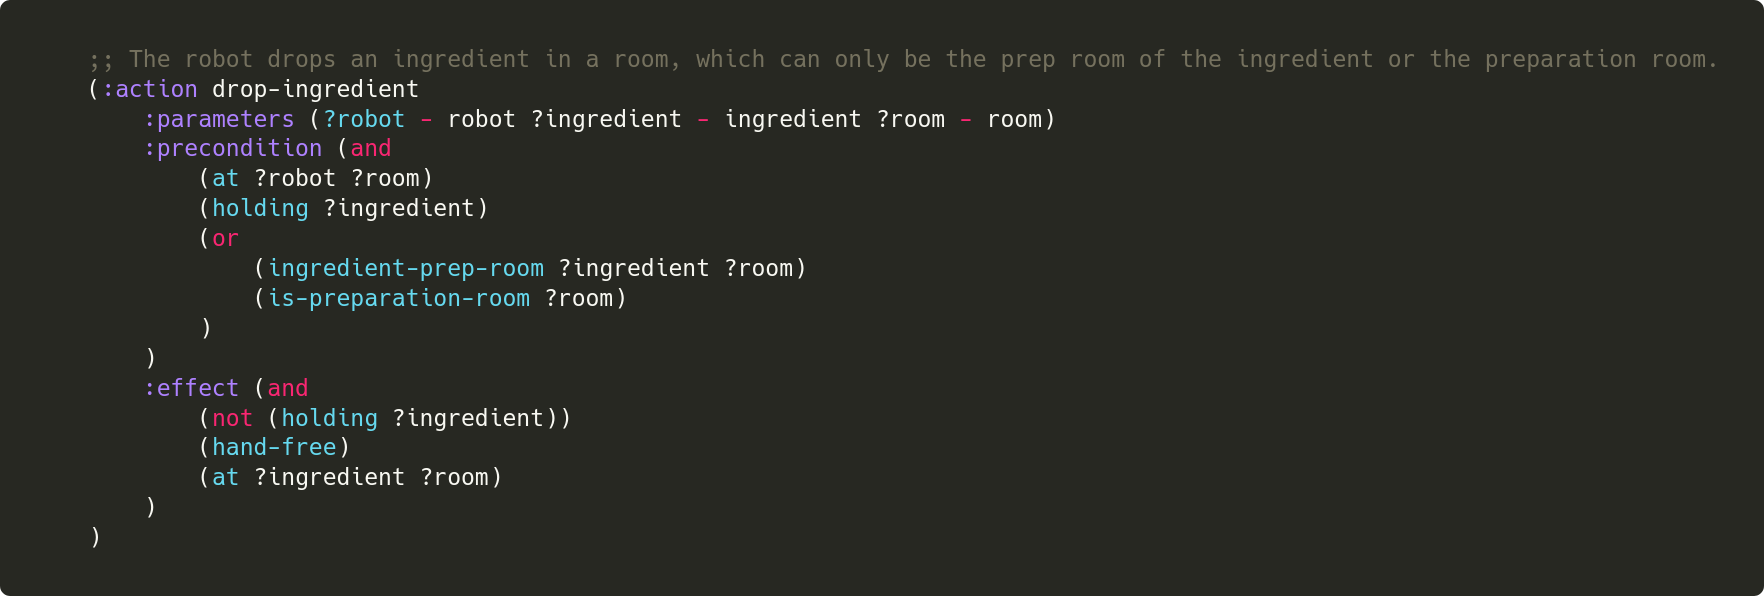
\includegraphics[width=0.90\textwidth]{assets/drop-ingredient.png}
    \caption{Code: Drop-ingredient Action}
    \label{fig:act:drop-ing}
\end{figure}

\subsubsection{Prepare-ingredient}
With the \texttt{prepare-ingredient} action, the robot prepares (cuts or mixes) an ingredient, depending on the designated preparation it requires.
\begin{itemize}
    \item \underline{Parameters:}
    \begin{itemize}
        \item \texttt{Robot}: The robot performing the preparation.
        \item \texttt{Ingredient}: The ingredient to be prepared.
        \item \texttt{Tool}: The tool required to prepare the ingredient.
        \item \texttt{Room}: The room where the ingredient is being prepared.
    \end{itemize}
    \item \underline{Preconditions:}
    \begin{itemize}
        \item \textit{At(Robot, Room)}: The robot must be located in the room \texttt{Room}.
        \item \textit{Ingredient-prep-room(Ingredient, Room)}: The ingredient must be prepared in this specified room.
        \item \textit{At(Ingredient, Room)}: The ingredient must be present in the room \texttt{Room}.
        \item \textit{Holding(Tool)}: The robot must be holding the required tool.
        \item \textit{Tool-use-room(Tool, Room)}: The tool must be usable in the specified room.
        \item \textit{Tool-clean(Tool)}: The tool must be clean before starting the preparation.
    \end{itemize}
    \item \underline{Effects:}
    \begin{itemize}
        \item \textit{Ingredient-prepared(Ingredient)}: The ingredient is now prepared.
        \item \textit{¬Tool-clean(Tool)}: The tool is no longer clean after preparing the ingredient.
    \end{itemize}
\end{itemize}
    \begin{figure}[H]
    \centering
    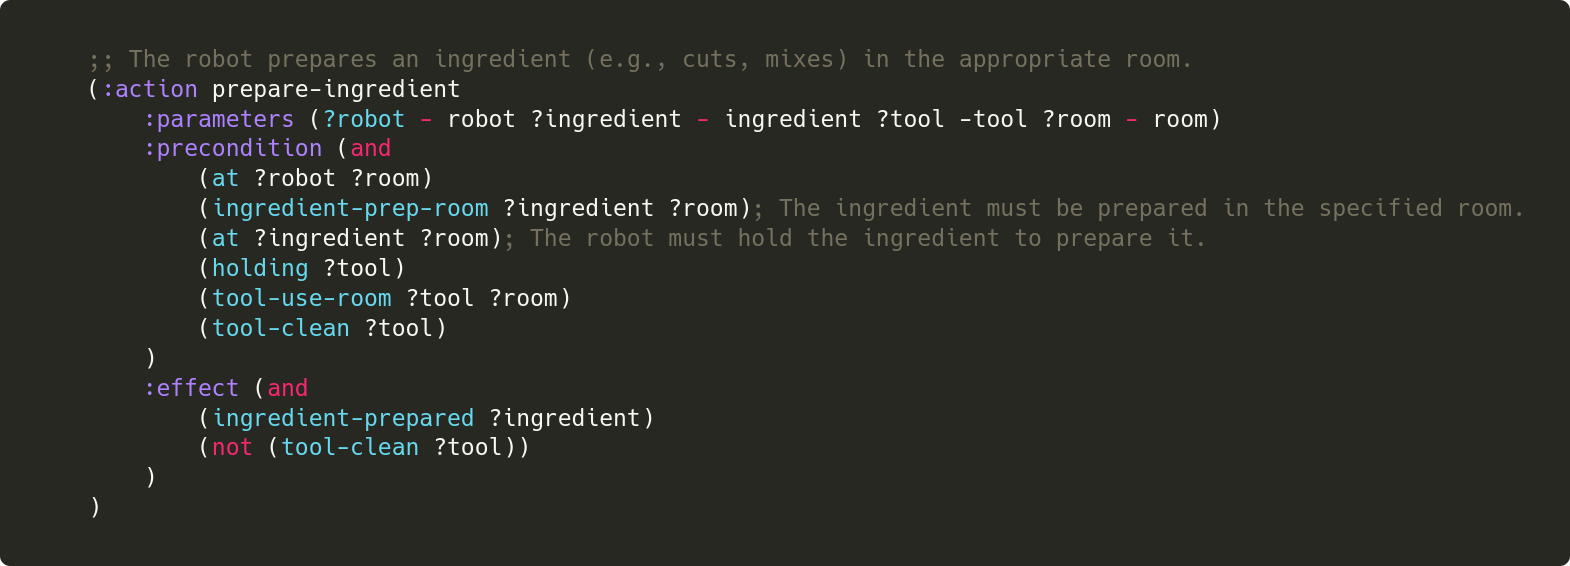
\includegraphics[width=0.90\textwidth]{assets/prepare-ingredient.png}
    \caption{Code: Prepare-ingredient Action}
    \label{fig:act:prepare-ing}
\end{figure}

\subsubsection{Cook-ingredient}
The \texttt{cook-ingredient} is used by the robot to cook an ingredient in the cooking room when it is required.
\begin{itemize}
    \item \underline{Parameters:}
    \begin{itemize}
        \item \texttt{Robot}: The robot performing the cooking action.
        \item \texttt{Ingredient}: The ingredient to be cooked.
        \item \texttt{Room}: The room where the cooking takes place.
    \end{itemize}
    \item \underline{Preconditions:}
    \begin{itemize}
        \item \textit{Is-cooking-room(Room)}: The room \texttt{Room} must be designated as a cooking room.
        \item \textit{At(Robot, Room)}: The robot must be located in \texttt{Room}.
        \item \textit{Ingredient-prepared(Ingredient)}: The ingredient must be prepared before it can be cooked.
        \item \textit{Holding(Ingredient)}: The robot must be holding the ingredient to cook it.
    \end{itemize}
    \item \underline{Effects:}
    \begin{itemize}
        \item \textit{Ingredient-cooked(Ingredient)}: The ingredient is now cooked.
    \end{itemize}
\end{itemize}
    \begin{figure}[ht]
    \centering
    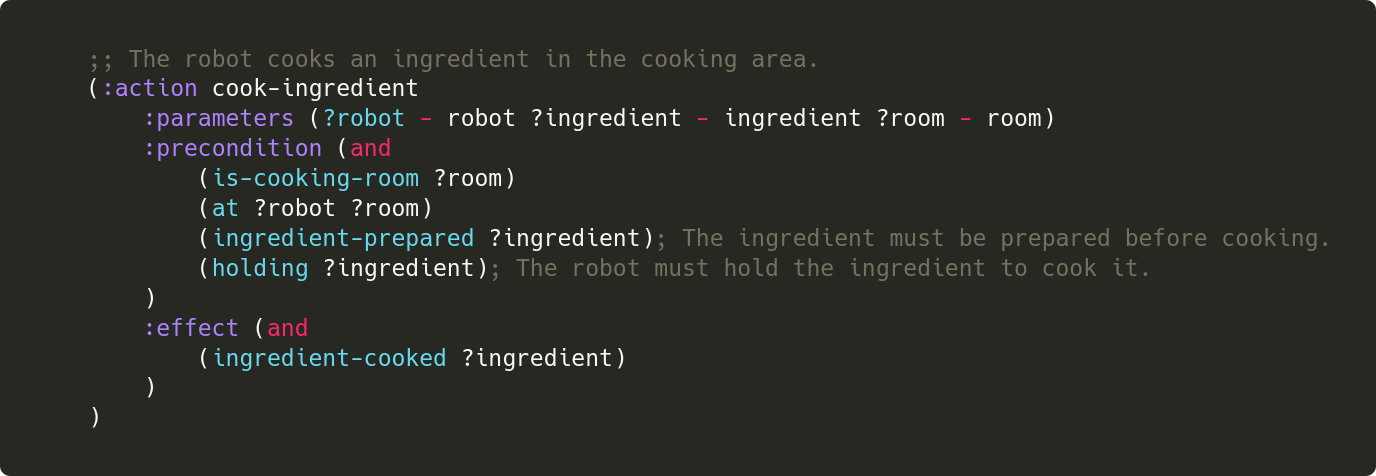
\includegraphics[width=0.90\textwidth]{assets/cook-ingredient.png}
    \caption{Code: Cook-ingredient Action}
    \label{fig:act:cook-ing}
\end{figure}

\subsubsection{Assemble-dish}
With the \texttt{assemble-dish} action, the robot is able to put together all of the prepared and/or cooked ingredients in order to produce a dish.
\begin{itemize}
    \item \underline{Parameters:}
    \begin{itemize}
        \item \texttt{Robot}: The robot responsible for assembling the dish.
        \item \texttt{Dish}: The dish being assembled.
        \item \texttt{Room}: The preparation room where the assembly takes place.
    \end{itemize}
    \item \underline{Preconditions:}
    \begin{itemize}
        \item \textit{At(Robot, Room)}: The robot must be located in \texttt{Room}.
        \item \textit{Is-preparation-room(Room)}: The room \texttt{Room} must be designated as the preparation area.
        \item \textit{Forall Ingredients}: Ensures all required ingredients meet the preparation requirements for the dish:
        \begin{itemize}
            \item If the dish requires a prepared ingredient, it must be \textit{Ingredient-prepared} and located in \texttt{Room}.
            \item If the dish requires a cooked ingredient, it must be \textit{Ingredient-cooked} and located in \texttt{Room}.
        \end{itemize}
    \end{itemize}
    \item \underline{Effects:}
    \begin{itemize}
        \item \textit{Dish-prepared(Dish)}: The dish is now prepared.
        \item \textit{At(Dish, Room)}: The dish is now located in \texttt{Room}.
        \item \textit{Forall Ingredients}: For each ingredient used in the dish:
        \begin{itemize}
            \item The ingredient is no longer available, prepared, or cooked.
            \item The ingredient is no longer located in \texttt{Room}.
        \end{itemize}
    \end{itemize}
\end{itemize}
    \begin{figure}[H]
    \centering
    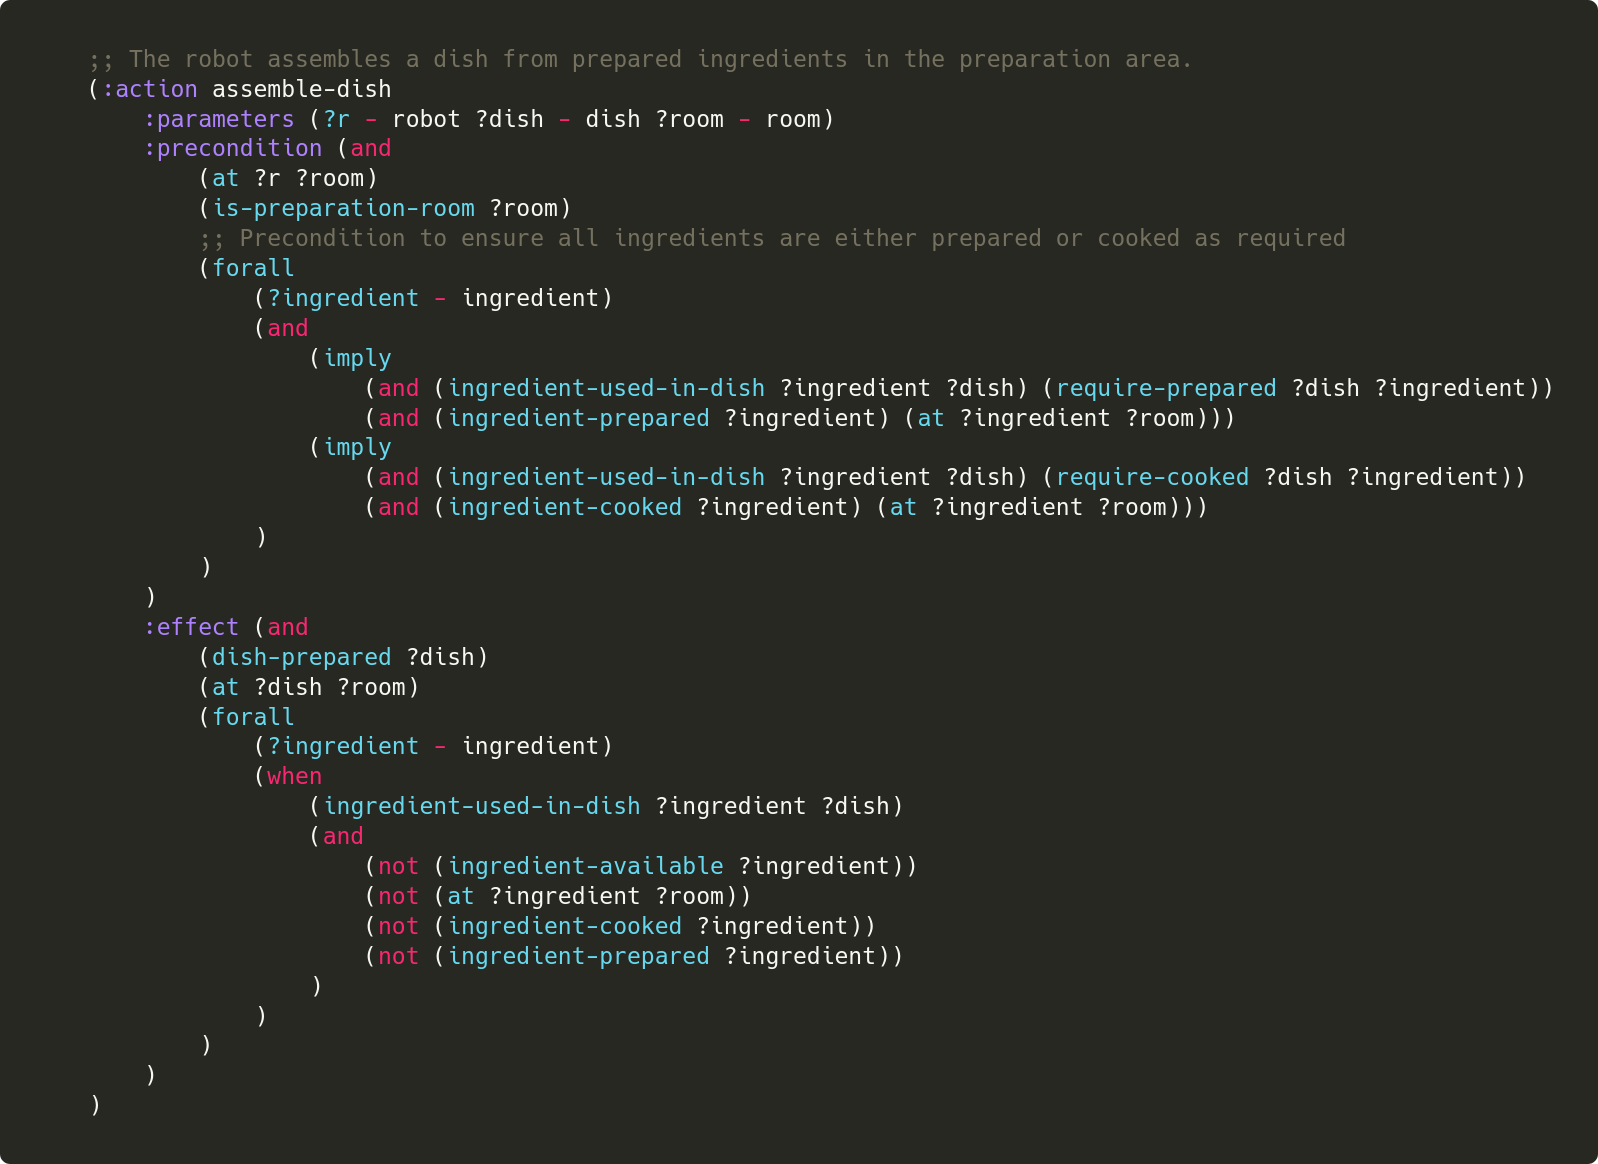
\includegraphics[width=0.90\textwidth]{assets/assemble-dish.png}
    \caption{Code: Assemble-dish Action}
    \label{fig:act:assemble-dish}
\end{figure}

\subsubsection{Serve-dish}
With the \texttt{serve-dish} action, the robot can finally serve a dish after it has been prepared.
\begin{itemize}
    \item \underline{Parameters:}
    \begin{itemize}
        \item \texttt{Robot}: The robot responsible for serving the dish.
        \item \texttt{Room}: The serving area where the dish is served.
        \item \texttt{Dish}: The dish to be served.
    \end{itemize}
    \item \underline{Preconditions:}
    \begin{itemize}
        \item \textit{Is-serving-room(Room)}: The room \texttt{Room} must be designated as the serving area.
        \item \textit{At(Robot, Room)}: The robot must be located in \texttt{Room}.
        \item \textit{Holding(Dish)}: The robot must be holding the dish.
        \item \textit{Dish-prepared(Dish)}: The dish must be fully prepared.
        \item \textit{Next-dish(Dish)}: The dish must be the next one in the serving order.
        \item \textit{Forall Other Dishes}: If there are any prioritized dishes before \texttt{Dish}, they must be served already.
    \end{itemize}
    \item \underline{Effects:}
    \begin{itemize}
        \item \textit{Dish-served(Dish)}: The dish is now marked as served.
        \item \textit{¬Holding(Dish)}: The robot is no longer holding the dish.
        \item \textit{Hand-free}: The robot’s hand is now free.
        \item \textit{¬Next-dish(Dish)}: The dish is no longer the next one in the serving order.
        \item \textit{Forall Other Dishes}: If \texttt{Dish} was prioritized before any other dish, that dish now becomes the next in line to be served.
    \end{itemize}
\end{itemize}
    \begin{figure}[ht]
    \centering
    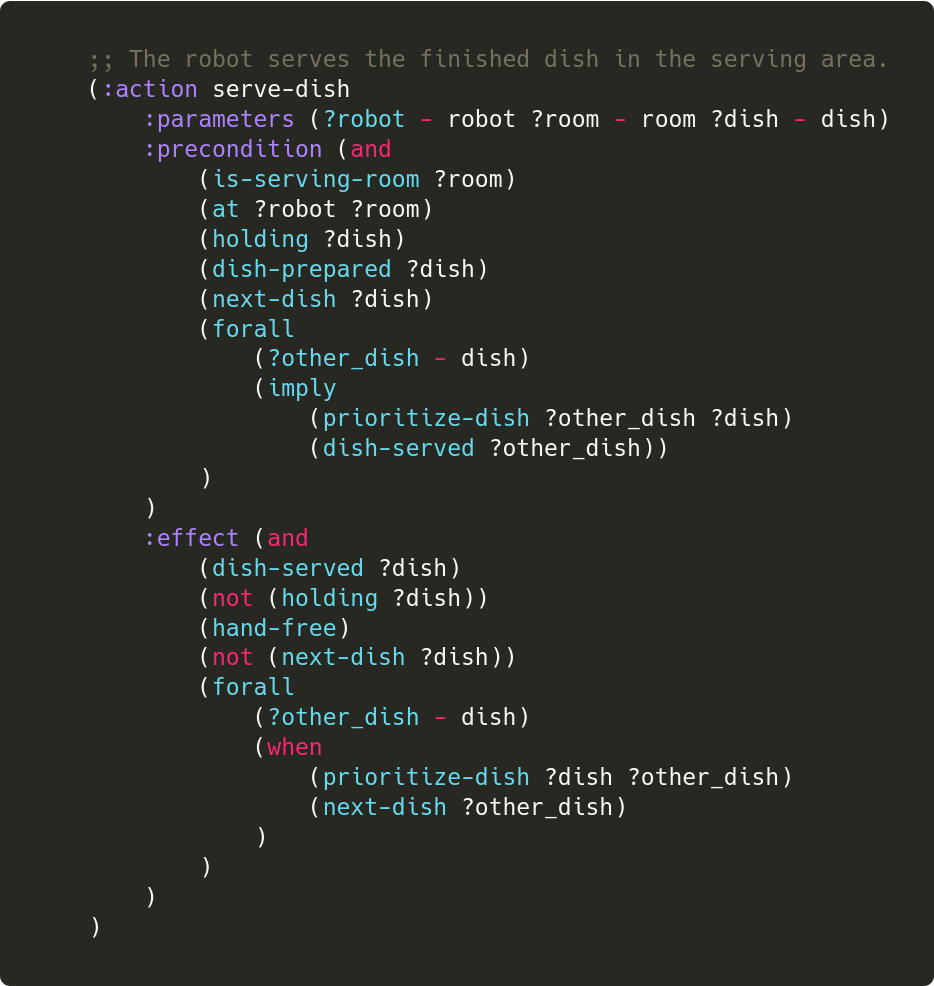
\includegraphics[width=0.70\textwidth]{assets/serve-dish.png}
    \caption{Code: Serve-dish Action}
    \label{fig:act:serve-dish}
\end{figure}

\newpage
\section{Test Cases and Results}

We conducted tests on a total of seven cases, each with increasing complexity. We began with a very basic scenario to verify the core functionality of the model and concluded with an unsolvable case that highlights the limitations of the established rules.

For each of the seven cases, we explain the objective of that test case, display a diagram of the initial and goal states, and briefly analyze the solution achieved with the planner. All of the solutions can be found in the \texttt{problem-*.plan} files attached to this report.

\subsection{Case 1: Basic}

To begin, we tested the fundamental functionalities of the model, focusing on the drone's basic movement and carrying actions. This initial test case features a small \(3 \times 3\) grid with no obstacles and a number of people that can comfortably fit into the safe zone.

\begin{figure}[ht]
    \centering
    %\includegraphics[width=0.55\textwidth]{assets/problem-1-basic.drawio.png}
    \caption{Case 1: Basic}
    \label{fig:initial-state}
\end{figure}
\FloatBarrier

We can see that the movement actions function correctly with the coordinate system we have built for the model, as well as the pick-up and drop-off actions.

\subsection{Case 2: Basic with Obstacles}

Subsequently, we incorporate an additional complexity into the model: the presence of obstacles. This scenario replicates the conditions of Case 1, utilizing a small grid and a number of individuals that can be accommodated within the safe zone. However, an obstacle is strategically positioned in the direct path between one of the individuals and the safe zone. This setup is designed to rigorously assess the drone's navigational algorithms and its ability to effectively circumvent obstacles.

\begin{figure}[H]
    \centering
    %\includegraphics[width=0.55\textwidth]{assets/problem-2-basic-obstacle.drawio.png}
    \caption{Case 2: Basic with Obstacles}
    \label{fig:initial-state-obstacles}
\end{figure}
\FloatBarrier

We now see that the obstacles also act as expected, impeding the movement actions through the cells they occupy. This makes the drone avoid the obstacle by moving around it.

\subsection{Case 3: Overcrowded}

For the next case, we examine another of the features of the model: the capacity of the safe zone. In order to do this, we again utilize a simple layout with a small grid and no obstacles, but in this case, we introduce one more person to rescue, which makes the total number of people bigger than the safe zone capacity. The goal of this test case is to study whether the “spots” feature of the safe zone works as expected.

\begin{figure}[H]
    \centering
    %\includegraphics[width=0.55\textwidth]{assets/problem-3-overcrowded.drawio.png}
    \caption{Case 3: Overcrowded}
    \label{fig:initial-state-overcrowded}
\end{figure}
\FloatBarrier

In this case, we prove that the safe zone capacity is being taken into account as it should, having to evacuate one of the spots before dropping off the last person at the safe zone.

\textbf{Note}: On earlier iterations of the model, we tried to implement the safe zone capacity with numeric functions (\texttt{:fluents} requirement of PDDL), but the available free online planners have trouble supporting them. Therefore, the concept of the spots of the free zone was implemented as a clean way to keep a count of the amount of people in the safe zone by only using predicates and actions (no functions)

\subsection{Case 4: Default (PDF example)}

For case 4, we evaluate the default scenario provided as an example in the assignment. This configuration involves rescuing three individuals and navigating around three obstacles within a \(4 \times 4\) grid. This test case is designed to assess nearly all aspects of the model's functionality within a slightly larger grid than previous scenarios.

\begin{figure}[ht]
    \centering
    %\includegraphics[width=0.55\textwidth]{assets/problem-4-pdf-example.drawio.png}
    \caption{Case 4: Default (PDF example)}
    \label{fig:initial-state-default}
\end{figure}
\FloatBarrier

It is now shown that we can easily enlarge the problem from a 3x3 to a 4x4 grid and the model still functions as expected.

\subsection{Case 5: Bigger Grid}

We proceed to conduct a test on a larger grid, specifically a \(5 \times 5\) configuration. This scenario includes five obstacles and six individuals requiring rescue, resulting in a situation where the number of people exceeds the available spots in the safe zone. This comprehensive test case is designed to evaluate all functionalities of the model within a single scenario.

\begin{figure}[ht]
    \centering
    %\includegraphics[width=0.55\textwidth]{assets/problem-5-big.drawio.png}
    \caption{Case 5: Bigger Grid}
    \label{fig:initial-state-bigger-grid}
\end{figure}
\FloatBarrier

Here we can appreciate how the most comprehensive test case (which includes all of the functionalities of the model) is solved correctly.

\subsection{Case 6: Maze}

With this test case, we aim to again display all of the functionalities of the model, but this time in a neat and visual scenario that simulates a maze.

\begin{figure}[ht]
    \centering
    %\includegraphics[width=0.55\textwidth]{assets/problem-6-maze.drawio.png} % Increased width
    \caption{Case 6: Maze}
    \label{fig:initial-state-maze}
\end{figure}
\FloatBarrier

We check again with a different test case that all of the functionalities behave as they should.

\subsection{Case 7: Impossible}

Finally, as a way to showcase the limits and restrictions of the model, we introduce a test case which is unsolvable. In this layout, the safe zone is fully surrounded by obstacles, and the only possible way to access it might be by moving diagonally, which is currently not an allowed type of movement.

\begin{figure}[H]
    \centering
    %\includegraphics[width=0.55\textwidth]{assets/problem-7-impossible.drawio.png} % Increased width
    \caption{Case 7: Impossible}
    \label{fig:initial-state-impossible}
\end{figure}
\FloatBarrier

Finally, we see how the planner indeed cannot find a solution to the proposed problem, which was the expected outcome, given that it should be impossible to solve with the given set of rules of the model

\section{Performance Analysis}

The following table summarizes the results of the test cases, comparing the performance metrics for the "Adjacency" and "Coordinates" approaches across different problems.

\begin{table}[ht]
    \centering
    \small
    \begin{tabular}{|c|l|c|c|c|c|}
        \hline
        \textbf{Problem} & \textbf{Method} & \textbf{Plan Cost} & \textbf{Nodes Generated} & \textbf{Nodes Expanded} & \textbf{Total Time} \\
        \hline
        \multirow{2}{*}{Problem-1} & Adjacency & 10 & 0 & 0 & 0.28 \\
                                   & Coordinates & 10 & 0 & 0 & 0.38 \\
        \hline
        \multirow{2}{*}{Problem-2} & Adjacency & 14 & 0 & 0 & 0.10 \\
                                   & Coordinates & 14 & 0 & 0 & 0.14 \\
        \hline
        \multirow{2}{*}{Problem-3} & Adjacency & 17 & 72 & 24 & 0.0308 \\
                                   & Coordinates & 17 & 57 & 18 & 0.1754 \\
        \hline
        \multirow{2}{*}{Problem-4} & Adjacency & 22 & 77 & 23 & 0.0320 \\
                                   & Coordinates & 22 & 725 & 248 & 1.6226 \\
        \hline
        \multirow{2}{*}{Problem-5} & Adjacency & 62 & 233 & 63 & 0.0172 \\
                                   & Coordinates & 62 & 46715 & 16940 & 1.8306 \\
        \hline
        \multirow{2}{*}{Problem-6} & Adjacency & 51 & 138 & 52 & 0.0149 \\
                                   & Coordinates & 51 & 10631 & 4749 & 3.9974 \\
        \hline
        \multirow{2}{*}{Problem-7} & Adjacency & - & 0 & 0 & 0.0007 \\
                                   & Coordinates & - & 0 & 0 & 0.0009 \\
        \hline
    \end{tabular}
    \caption{Comparison of performance metrics for different solutions and problems.}
    \label{tab:results}
\end{table}

The table evaluates the following several key performance metrics for each approach:

\begin{itemize}
    \item \textbf{Plan Cost:} Represents the cumulative cost of executing all actions in a plan. Lower costs indicate more efficient solutions.
    
    \item \textbf{Nodes Generated:} Provides insight into the computational effort of the search algorithm by indicating the total number of states considered.
    
    \item \textbf{Nodes Expanded:} Shows how many of the generated states were fully explored, offering a measure of the search's thoroughness.
    
    \item \textbf{Total Time:} Reflects the duration taken by the algorithm to find a solution. Faster times are advantageous, especially in time-sensitive scenarios.
\end{itemize}

Our results provide a comparative analysis of the "Adjacency" and "Coordinates" approaches across several problems. The Plan Cost remains consistent across both approaches for each problem, indicating that both methods are equally effective in terms of the cost of executing actions. Notably, in Problems 1 and 2, the metrics for Nodes Generated and Nodes Expanded are both zero. This suggests that these problems are straightforward enough that the initial state is already close to the goal state, requiring minimal exploration of the search space. Consequently, the search algorithms can directly reach the solution without generating or expanding additional nodes. However, as the complexity of the problems increases, the "Coordinates" approach generally generates and expands more nodes than the "Adjacency" approach, particularly noticeable in Problems 4 and 5. This indicates that the "Coordinates" method explores a larger search space, which could imply a more thorough search and therefore more computational effort. Interestingly, in Problem 3, the "Coordinates" solution generated and expanded fewer nodes than the "Adjacency" approach, yet it was still significantly slower. This highlights a potential inefficiency in the "Coordinates" method, where even with fewer nodes, the time taken is longer. The Total Time metric consistently shows that the "Coordinates" approach often takes longer to find a solution compared to the "Adjacency" approach. This is especially evident as the complexity of the problems increases, where the time difference becomes more pronounced. Overall, the "Adjacency" approach appears to be more efficient in terms of computational resources and time, particularly as the complexity of the problem evolves.

\newpage
\section{Conclusion}

In this report, we explored two distinct approaches for modeling a rescue drone tasked with saving individuals in an emergency grid environment: the "Adjacency List" and the "Coordinate System" methods. Through a series of test cases, we evaluated the performance of each approach in terms of Plan Cost, Nodes Generated, Nodes Expanded, and Total Time.

\vspace{1em}

Our analysis revealed that while both approaches achieve optimal Plan Costs, the "Adjacency List" method consistently outperforms the "Coordinate System" in terms of computational efficiency, particularly as the complexity of the problems increases. This is evidenced by the lower number of nodes generated and expanded, as well as the reduced total time required to find solutions. The "Coordinate System" approach, although more concise in its problem definition, tends to explore a larger search space, leading to increased computational effort and time.

\vspace{1em}

Interestingly, in simpler scenarios such as Problems 1 and 2, both methods required minimal exploration, resulting in zero nodes generated and expanded. However, as the complexity increased, the "Adjacency List" approach demonstrated superior efficiency, making it a more suitable choice for complex problem-solving scenarios.

\vspace{1em}

This study emphasizes the importance of selecting the right modeling approach based on the specific needs and constraints of the problem to achieve the best results effectively and efficiently. Additionally, exploring the use of fluents or comparing our methods with other planners could provide further insights and improvements.

\end{document}